\documentclass[a4paper]{article}
% \documentclass[a4paper,twoside]{article}
\usepackage[utf8]{inputenc}
\usepackage[T1]{fontenc}
\usepackage{amsmath}
\usepackage{mathtools}
\usepackage{standalone}
\usepackage{float}
\usepackage{subcaption}
\usepackage{multirow}

% \usepackage[english]{babel}
% \usepackage[square,sort,comma,numbers]{natbib}
% \usepackage{babelbib}
% \bibliographystyle{babplain}


\title{Thesis: Really Important Stuff}
\author{Max Mustermann}

\begin{document}
  \maketitle

  \documentclass[crop=false]{standalone}

\begin{document}
  \begin{abstract}
    Lorem ipsum dolor sit amet, consectetur adipisicing elit, sed do eiusmod
    tempor incididunt ut labore et dolore magna aliqua. Ut enim ad minim veniam,
    quis nostrud exercitation ullamco laboris nisi ut aliquip ex ea commodo
    consequat. Duis aute irure dolor in reprehenderit in voluptate velit esse
    cillum dolore eu fugiat nulla pariatur. Excepteur sint occaecat cupidatat non
    proident, sunt in culpa qui officia deserunt mollit anim id est laborum.
  \end{abstract}
\end{document}

  \tableofcontents
  \cleardoublepage
  \listoffigures

  % \newpage
  \cleardoublepage

  \documentclass[crop=false]{standalone}

\begin{document}
  \begin{abstract}
    Lorem ipsum dolor sit amet, consectetur adipisicing elit, sed do eiusmod
    tempor incididunt ut labore et dolore magna aliqua. Ut enim ad minim veniam,
    quis nostrud exercitation ullamco laboris nisi ut aliquip ex ea commodo
    consequat. Duis aute irure dolor in reprehenderit in voluptate velit esse
    cillum dolore eu fugiat nulla pariatur. Excepteur sint occaecat cupidatat non
    proident, sunt in culpa qui officia deserunt mollit anim id est laborum.
  \end{abstract}
\end{document}

  \section{Introduction}
    \begin{figure}[H]
      \center
      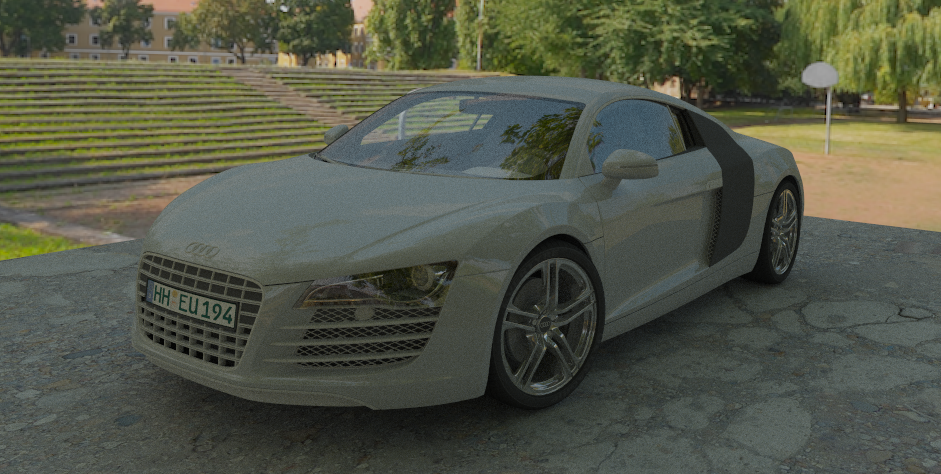
\includegraphics[width=0.9\textwidth]{example-audi_r8-pt.png}
      \caption[Audi Car]{This figure shows a cool car!}
      \label{fig:audi}
    \end{figure}

    The figure \ref{fig:audi} shows a cool car which was generated by the computer.

  \section{Background}
    \begin{figure}[H]
      \center
      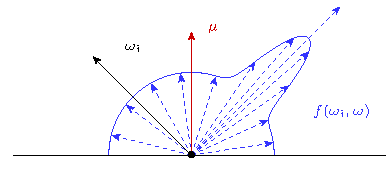
\includegraphics[width=0.9\textwidth]{brdf_1.pdf}
      \caption{This one is a scheme.}
      \label{fig:brdf}
    \end{figure}

  \section{Methodology}
    \begin{figure}
      \center
      \begin{subfigure}[b]{0.49\textwidth}
        \center
        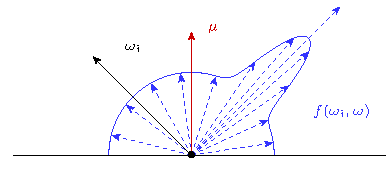
\includegraphics[width=0.9\textwidth]{brdf_1.pdf}
        \caption{first}
      \end{subfigure}
      \begin{subfigure}[b]{0.49\textwidth}
        \center
        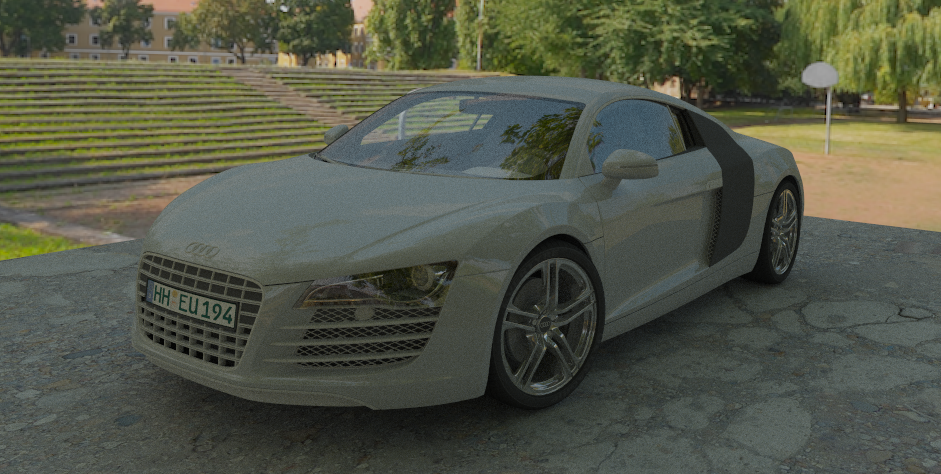
\includegraphics[width=0.9\textwidth]{example-audi_r8-pt.png}
        \caption{second}
      \end{subfigure}

      \begin{subfigure}[b]{0.99\textwidth}
        \center
        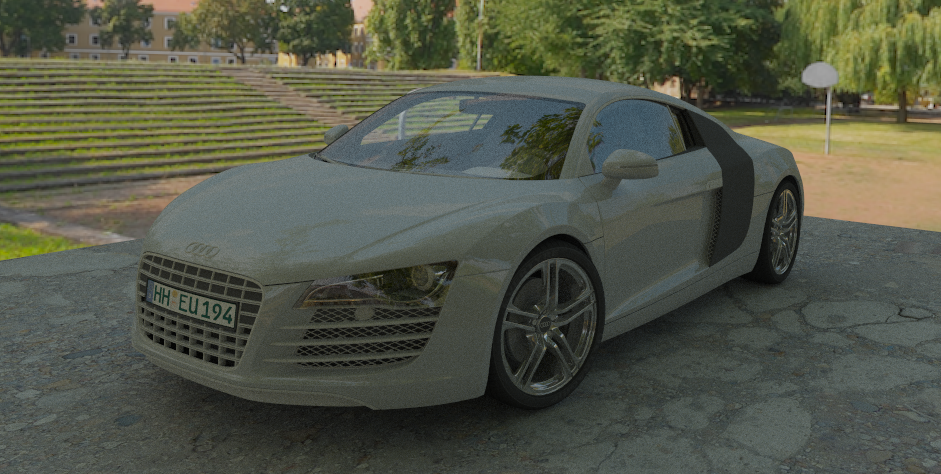
\includegraphics[width=0.9\textwidth]{example-audi_r8-pt.png}
        \caption{third}
      \end{subfigure}
      \caption[Wow!]{Two images!}
    \end{figure}

  \section{Implementation}
  \section{Measurement}
  \section{Results}

    \begin{table}[H]
      \center
      \caption{testtable}
      \begin{tabular}{llll}
        \hline
        One & Two & Three & Four \\
        \hline
        \hline
        1 & 2 & 3 & 4 \\
        text & more text & only text & nah... \\
        \hline
      \end{tabular}
    \end{table}

    \begin{table}[H]
      \center
      \caption{testtable}
      \begin{tabular}{lrcl}
        \hline
        One & Two & Three & Four \\
        \hline
        \hline
        1 & 2 & 3 & 4 \\
        text & more text & only text & nah... \\
        \hline
      \end{tabular}
    \end{table}

    \begin{table}[H]
      \center
      \caption{testtable}
      \begin{tabular}{|l|r|cl|}
        \hline
        One & Two & Three & Four \\
        \hline
        \hline
        1 & 2 & 3 & 4 \\
        text & more text & only text & nah... \\
        \hline
      \end{tabular}
    \end{table}

    \begin{table}[H]
      \center
      \begin{tabular}{lll}
        \hline
        one & two & three \\
        \hline
        \hline
        \multirow{2}{*}{$n$} & $p$ & $q$ \\
          & $a$ & $b$ \\
        \hline
      \end{tabular}
    \end{table}

    \begin{table}[H]
      \center
      \begin{tabular}{lll}
        \hline
        one & two & three \\
        \hline
        \hline
        \multirow{2}{*}{$n$} & \multirow{2}{*}{$p$} & $q$ \\
          & & $b$ \\
        \hline
      \end{tabular}
    \end{table}

  \section{Conclusion}

  % \nocite{*}
  % \bibliography{references}

  \appendix
  \section{Extra Results}
  \section{More Background}
\end{document}